\chapter{Capture and Replay for Eiffel}
\eiffellisting
\section{Differences to Existing Implementation}
Selective capture and replay as described by Joshi and Orso \cite{orso05may} can not be directly applied to Eiffel. Although the core elements of the technique can be used in Eiffel, too, we need to adapt some parts. In this section the changes to the original implementation and reasons for these changes will be discussed.

\subsection{Language Aspects}
Even though Java and Eiffel are both object oriented languages, there are differences between these two languages, syntax left aside. Eiffel offers a wider set of language constructs, many times trying to solve problems inherently object oriented, whereas Java reused solutions from its ancestors, mainly C++. One example for this difference could be the Eiffel basic types, which can be treated as objects with methods and attributes versus the Java basic types, which are no objects. This section focuses on the differences between Java and Eiffel that influenced our implementation of selective capture and replay.

\subsubsection{Terminology} % diesen Titel weglassen?
Eiffel has a nomenclature that differs from other programming languages. Here the Eiffel terminology is described according to \cite{oosc2} and compared to the one from Java.
\begin{center}
\begin{tabular}[]{|l|l|} \hline
 \textbf{Eiffel}&\textbf{Java} \\ \hline
 Attribute&Field \\ \hline
 Ouery&Field or Method that has a return value \\ \hline
 Routine&Method \\ \hline
 Procedure&Method that has no return value \\ \hline
 Function&Method that has a return value \\ \hline
 Feature&Method or Attribute \\ \hline
 ANY&Object (ancestor of all classes) \\ \hline
\end{tabular} 
\end{center}

\subsubsection{Multiple Inheritance}
Eiffel is designed to support multiple inheritance, whereas in Java, only single inheritance is allowed. The original implementation assumes, that all subclasses of a class \emph{c} are in the observed set iff \emph{c} is also in the observed set. This makes it possible to statically decide whether an observed or an unobserved feature is accessed.

If this assumption is translated to multiple inheritance, it would not be possible to have a class \emph{C} that inherits both from an observed class \emph{A} and an unobserved class \emph{B} (\figref{fig:obs_unobs_multiple_inheritance}).
\begin{figure}[ht]
  \centering
  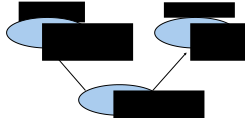
\includegraphics[width=0.5\textwidth]{illustrations/obs_unobs_multiple_inheritance}
  \caption{Conflict Due to Multiple Inheritance}
  \label{fig:obs_unobs_multiple_inheritance}
%\includegraphics{illustrations/capture_and_replay_generic_structure}
\end{figure}

Multiple inheritance is extensively used in Eiffel, thus this assumption would be too restrictive in our opinion. It would lead to big clusters that could not be divided into observed and unobserved set. 

Although Java does not allow multiple inheritance, it supports multiple interface inheritance. Joshi and Orso \cite{orso05may} mention that they need to dynamically determine if the target of an event is observed or unobserved in certain cases. We assume that multiple interface inheritance with a class that both implements an observed and unobserved interface  is at least one of these cases. They use the \texttt{instanceof} operator determine if an object is an instance of an observed class.

We will present a solution that always determines dynamically, if an object is an instance of an observed class (\emph{observed object}) or an instance of an unobserved class (\emph{unobserved object}), together with a proposal how to solve this problem without reflection.

\subsubsection{Read Only Attributes}
Eiffel strictly follows the \emph{uniform access principle} \cite{oosc2}. The principle states that it should not be visible to the clients whether features are implemented through storage or computation. This ensures that the implementation of a feature could be changed from attribute to function or vice versa. One of the consequences of this principle is that clients of a class cannot write to attributes, as these attributes could be implemented as a function as well.

In Java, this principle is not ensured because clients of a class can write to their fields. For our implementation of selective capture and replay, this limits the events related to field accesses to OUTREAD. Both OUTWRITE and INWRITE can not happen, because write access to fields is restricted to their class, thus there can not be any write accesses to fields from observed to unobserved classes or reverse.

\subsection{Target Application}
As a first application that could use selective capture and replay in Eiffel, Cdd, a tool for Contract Driven Development \cite{cdd07} was chosen. Cdd allows programmers to extract test cases from failing program runs. The contracts that are present in the code are used as test oracles.Cdd is not always able to generate such a test case, due to different reasons:

\begin{description}
\item [Prestate extraction:] The state before calling the failing feature (which is needed to generate a test case) is extracted using the state at the time of failure. Because not all instructions between feature call and failure can be undone, the extraction of the prestate is not always possible.
\item [Non-determinism:] If the failing feature reads values from sources that don't always return the same values (eg. user input), it's not generally possible to run the test cases with the same result as in the failing run.
\item [External state:] When the feature relies on state that is not stored in Eiffel objects (e.g. in C structs), Cdd is not able to gather this state for the test.
\end{description}

All these limitations can be resolved using selective capture and replay:
\begin{description}
\item [Prestate extraction:] By setting a breakpoint at the beginning of the failing feature, it is possible to extract the prestate during the replay of the application.
\item [Non-determinism:] When adding all non-deterministic classes to the unobserved set, it can be ensured that the replay of the run is deterministic.
\item [External State:] All classes that wrap external state can be added to the unobserved set. Thus interactions with these classes can be replayed without having to store the external state.
\end{description}

Prestate extraction using selective capture and replay requires an immediate rerun of the application under test. Because complete recompiles in Eiffel last for tens of minutes up to hours, we can not afford to instrument the application again before replaying it. Thus it is necessary to design the code instrumentation to be both applicable for capture and replay phase. We pushed this approach even further to allow the user to disable the whole instrumentation. This allows execution with minimal overhead if capture and replay is not needed without recompiling the application.

\section{Code Instrumentation}
\subsection{Outline}
Due to differences between Eiffel and Java and a different use case, there are two main differences between the original implementation and our approach:

\begin{enumerate}
 \item It is necessary to determine dynamically whether an object is observed or not.
\item It must be possible to switch between capture and replay phase without reinstrumenting the code.
\end{enumerate}

The first requirement can be met by adding an additional query to every class so that it is possible to find out whether an object is an instance of an observed or an unobserved class. We ensure that every class has this query by adding it to ANY. In the next chapter we will discuss how this query can be implemented efficiently.

In order to be able to switch between capture and replay mode, the class PROGRAM\_FLOW\_SINK was introduced. Program flow events are put into the PROGRAM\_FLOW\_SINK. It is both the ancestor class of RECORDER, the class that contains the management code for recording events and PLAYER, the class that provides the scaffolding for replaying events. The standard instance of a PROGRAM\_FLOW\_SINK is globally accessible. It is dynamically bound to an instance of RECORDER during capture phase and PLAYER during replay phase.

To create placeholder objects from unobserved classes, their original routine bodies are disabled during replay pha phase. When replaying, the routines only execute instrumentation code that invokes the scaffolding and takes care of the return value if necessary.

\subsection{Routines}
Whereas the original implementation captures routine calls by instrumenting the call site (in the client), we decided to instrument the calee (the supplier). This simplifies code instrumentation, because there is no need to make changes inside existing routine bodies, it is sufficient to add some code at the beginning and the end of the routine bodies. %TODO Gibt es noch ein besseres Motiv?

The routine instrumentation can be divided into three parts (\figref{fig:routine_instrumentation_structure}): Right at the beginning of the routine, code to detect call events is inserted. The original routine body is made conditional so that it is not executed for unobserved routines during the replay phase. Finally, code to detect callret events is inserted at the end of the routine.
\begin{figure}[ht]
  \centering
  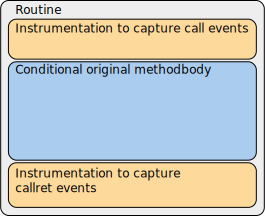
\includegraphics[width=0.5\textwidth]{illustrations/routine_instrumentation_structure}
  \caption{Structure of Routine Instrumentations}
  \label{fig:routine_instrumentation_structure}
\end{figure}

To explain instrumentation in more detail, we describe each of these three parts using the command \texttt{withdraw} of the class \texttt{ATM} (\listref{lst:withdraw_original}).

\begin{lstlisting}[caption=Original Code of Command \texttt{withdraw} ,label=lst:withdraw_original]
withdraw (account_name: STRING_8; amount: REAL_32)
		-- Withdraw 'amount' on the account with name 'account_name'
	require
		account_exists: account_exists (account_name)
	local
		an_account: BANK_ACCOUNT
	do
		an_account := the_bank.account_for_name (account_name)
		if an_account /= Void then
			the_bank.withdraw (an_account, amount)
			success := True
		else
			success := False
		end
	end
\end{lstlisting}

\subsubsection{Capturing Call Events}
\subsubsection{Conditional Methodbody Execution}
\subsubsection{Capturing Callret Events}



\begin{itemize}
 \item Code to detect call events (INCALL and OUTCALL) is inserted right at the beginning of the routine. If a border crossing call is detected, the code prepares the routine arguments, the target of the call and the routine name for the PROGRAM\_FLOW\_SINK.
 \item The technique makes sure that the original method body of unobserved routines is only executed during capture phase.
 \item After the conditional method body, instrumentation code to detect the callret events (INCALLRET and OUTCALLRET) follows. If the call was triggered across the border, the return value is prepared for the PROGRAM\_FLOW\_SINK.
\end{itemize}




\begin{lstlisting}
withdraw (account_name: STRING_8; amount: REAL_32)
		-- Withdraw 'amount' on the account with name 'account_name'
	require
		account_exists: account_exists (account_name)
	local
		an_account: BANK_ACCOUNT
		ignore_result: ANY
	do
		if program_flow_sink.is_capture_replay_enabled then
			program_flow_sink.enter
			if program_flow_sink.observed_stack_item /= is_observed then
				program_flow_sink.put_to_observed_stack (is_observed)
				program_flow_sink.put_feature_invocation ("withdraw", Current, [account_name, amount])
			else
				program_flow_sink.put_to_observed_stack (is_observed)
			end
			program_flow_sink.leave
		end
		if (not program_flow_sink.is_replay_phase) or is_observed then
			an_account := the_bank.account_for_name (account_name)
			if an_account /= Void then
				the_bank.withdraw (an_account, amount)
				success := True
			else
				success := False
			end
		end
		if program_flow_sink.is_capture_replay_enabled then
			program_flow_sink.enter
			program_flow_sink.remove_from_observed_stack
			if program_flow_sink.observed_stack_item /= is_observed then
				program_flow_sink.put_feature_exit (Void)
			end
			program_flow_sink.leave
		end
	end
\end{lstlisting}



The problem arises, because the management code uses the same libraries as the application. When for example RECORDER writes an event to a file, this should not trigger additional events.  

\subsection{Attribute Accesses}
\subsection{Attribute Manipulation from C Level}



\section{Architecture}
%unterschiedliche Parts noch genauer beschreiben
%-Log: (mikro-architektur), wieso kein XML?
\section{Advantages over Traditional Capture and Replay}
\section{Limitations}
%unter welchen Umstaenden musste manuell instrumentiert werden??
\section{Future Steps}
%Fehlende features + idee zu deren implementierung

\section{Building the Example from Source}
In this section the process of building an example with capture replay support under Linux will be described. Setting up the modified version of Eiffel Studio and all necessary tools will take the biggest part of this explanation.\\
%TODO: wieso genau wird eine modifizierte Version von Eiffel Studio benoetigt??
It is assumed that all commands in the following steps are executed in the same session, thus keeping the environment variables.\\

\subsection{Building the Preliminaries}
The first tools we need are the  Eiffel Studio Tools \cite{estudiotools}. These will be used in many setup scripts in the examples or tests from the repository. Install those tools according to the description on the webpage.\\

The delivery of the modified Eiffel Studio was built using revision 69201 of Eiffel Studio. Building a delivery with a later version of Eiffel Studio was not testet, so it might not work. If no binaries of revision 69201 are available, a delivery of that revision from source \texttt{(stimmt das wirklich??? gaebe das kein Henne / Ei Problem?)}.\\
After copying the delivery to ~/estudio/Eiffel60\_gpl\_69201, it can be activated:
\bashlisting
\begin{lstlisting}
   activate_estudio 60_gpl_69201
\end{lstlisting}

Now Gobo \cite{gobo} can be installed can be installed from svn (Revision 6001 was successfully tested).
- Install Gobo  from svn (revision 6001) -->
\begin{lstlisting}
svn co -r6001 https://gobo-eiffel.svn.sourceforge.net/svnroot/gobo-eiffel/gobo/trunk ~/capture_replay/gobo
export GOBO=~/capture\_replay/gobo
export PATH=$GOBO/bin:$PATH
$GOBO/work/bootstrap/bootstrap.sh gcc ise
\end{lstlisting}

As all preliminaries are installed, Erl-G \cite{erlg} can be downloaded and built. Revision 719 of Erl-G was tested together with capture and replay.
\begin{lstlisting}
svn co -r719 https://svn.origo.ethz.ch/autotest/trunk/erl_g ~/capture_replay/erl_g
export ERL_G=~/capture_replay/erl_g
export PATH=$ERL_G/bin:$PATH
cd $ERL_G
#EIFFEL_SRC is needed. avoid conflicts between EIFFEL_SRC and ISE_LIBRARY.
export ISE_LIBRARY=$EIFFEL_SRC
geant install
geant compile
\title{Selective Capture and Replay for Eiffel
\end{lstlisting}

To build a delivery of the modified Eiffel Studio, execute these commands: (this will take a few hours).
\begin{lstlisting}
cd ~/capture_replay/
mkdir es
svn co https://eiffelsoftware.origo.ethz.ch/svn/es/branches/capture_replay es
export EIFFEL_SRC=~/capture_replay/es/Src
cd es
geant -b $EIFFEL_SRC/scripts/build.eant build_es
\end{lstlisting}

Before an example can be built the delivery that was just created needs to used be set as default instance of Eiffel Studio
\begin{lstlisting}
cd ~/estudio
ln -s ~/capture_replay/es/EiffelXX EiffelCR
activate_estudio CR
\end{lstlisting}

In order to make the created Eiffel Studio use a modified version of the runtime, it is necessary to recompile the runtime with modified CFLAGS. The new version of the runtime then needs to be installed in the delivery.

It is not possible to directly build Eiffel Studio with the modified version of the runtime, because the changes in the runtime are not compatible to Eiffels store mechanism (\texttt{TODO: das auch noch unter irgendwelchem future work anmerken...}). This would render Eiffel Studio unusable because it relies on this mechanism during the build process.
\begin{lstlisting}
export CFLAGS='-DCAPTURE_REPLAY' 
cd $EIFFEL_SRC
#build the runtime from scratch (clobber the old one)
geant -b scripts/build.eant compile_runtime
cd $ISE_EIFFEL/studio/spec/linux-x86/lib
rm *
cp $EIFFEL_SRC/C/run-time/lib* .
\end{lstlisting}


\subsection{Building an Example}
Now, all necessary tools should be installed and the corresponding environment variables set. And we can start to build an example.\\
First we need to add reflection support to the example project. Erl G will generate reflection classes for us. If the environment variables are correctly set, the geant script should invoke Erl G automatically. \\
At the moment Erl-G does not support overrides because this feature is missing in the Gobo parser. Therefore it's necessary to override the necessary classes manually. There are two geant tasks that take care of this:

\begin{itemize}
\item \identifier{patch\_elks} makes the manual override by copying the modified elks classes from \$EIFFEL\_SRC/library/base/capture\_replay/elks\_overrides to \$ISE\_LIBRARY/library/base/elks \\
\item \identifier{unpatch\_elks} restores the original state by copying the original elks classes from \$EIFFEL\_SRC/library/base/elks to \$ISE\_LIBRARY/library/base/elks .
\end{itemize}

\begin{lstlisting}
cd ~/capture_replay/es/examples/capture_replay/iteration1
geant install
\end{lstlisting}

The example can now be opened with the modified version of Eiffel Studio. Make sure that the CFLAGS are still set to '-DCAPTURE\_REPLAY'. Otherwise it will not be possible to build the example.



\section {Limitations}
%-Konstruktoren nach ANY exportiert (fehlende unterstuetzung von Eiffel-Seite fuer Konstruktoren)
%- Access modifiers e.g. export of a observed feature only to an unobserved class --> replay not possible.